% Author: Pavol Loffay
% Project: Master thesis - Hawkular alert prediction
% Date 20.2.2015

\chapter{Introduction} 
An Alert prediction is very important because it can predict critical states of a system in
advance. It gives system administrators powerful feature to reduce for instance downtime
of an application or ability to load balance workload in advance.
TODO

\section{Context}
The implementation part of the master thesis is developed as part of the project
Hawkular\footnote{Available at \url{http://www.hawkular.org}}. 
Therefore the application architecture and used technologies had to fit 
into the overall project environment.

Hawkular is an open source monitoring and management platform mainly
developed by company Red Hat. It is successor of very successful RHQ
project\footnote{Available at \url{https://rhq-project.github.io/rhq/}}.
This application is designed to monitor Java application servers
like Wildfly, Apache Tomcat and other middleware systems. 
For instance it can monitor heap usage, web sessions, used data sources etc.

TODO describe more Hawkular - modules(mention scalability), metrics structure

\section{Goals}
The main goal of the application is to provide users with reliable predictions
of alerts for the set of collected metrics. Displaying of forecast is also very
important and should be available in the user interface. This feature can help 
system administrators react on events like running out of memory well
in advance.

TODO performance(loads of metrics), 

%%%%%%%%%%%%%%%%%%%%%%%%%%%%%%%%%%%%%%%%%%%%%%%%%%%%%%%%%%%%%%%%%%% 
\chapter{Time Series Analysis}
In this chapter are discussed various approaches for forecasting time series and
also relevant theory which is helpful for understanding them.
Models are ordered from simpler to more complex ones. 

In the early part of the thesis
development system R was used for quickly showing the results of forecasts and also 
for better understanding metric data by plotting it.

Firstly it is important to define time series; it is sequence of observations
$ s_t \in \mathbb{R} $ usually ordered in time. In this thesis are used only
equidistant discrete univariate time series. 

Forecasting is a process of making prediction of the future based 
on the past. In other words forecasting is possible because  
future depends on the past or analogously because there is a relationship
between the future and the past. However this relation is not deterministic and 
can be hardly written in an analytical form.

There are two forecasting types: qualitative and quantitative.
Qualitative methods are mainly based on the opinion of the subject and are used 
when past data are not available, hence not suitable for this project. 
When there are past data available quantitative forecasting methods are more suitable. 

\section{Simple quantitative methods}
There are three simple quantitative forecasting methods:

\begin{itemize}
    \item Average method\,--\,forecasts are equal to the value of the mean of
        historical data.
        $$ \hat{y}_{T+h|T} = \overline{y} = (y_{1}+ \dots + y_{T}) / T $$
    \item Na\"{i}ve method\,--\,forecasts are equal to the last observed value.
        $$ \hat{y}_{T+h|T} = y_{T} $$ 
    \item Drift method\,--\,variation of na\"{i}ve method which allow the
        forecasts to increase or decrease over time.
        $$ \hat{y}_{T+h|T} = y_{T} + \frac{h}{T-1} \sum_{t=2}^T{y_{t} - y_{t-1}} = 
        y_{T} + h(\frac{y_{T}-y_{1}}{T-1}) $$
\end{itemize}
There is also an seasonal variant of na\"{i}ve method. This method is suitable only
for highly seasonal data. Forecast is simply equal to last observed value from
the previous season.

\section{Time series decomposition}
In the time series can be seen various patterns(TODO ref otext). It is crucial to categorize
some of them. Basic observed patterns are trend, seasonality, cycle and irregular
component also called white noise. 

\begin{itemize}
    \item \textbf{Trend $ T_{t} $}\,--\,exists if there is long term increase or decrease over
        time. Can be linear or nonlinear (e.g. exponential growth)
    \item \textbf{Seasonal $ S_{t} $}\,--\,exists when a series is influenced by seasonal factors.
        Seasonality is always of fixed and known period.
    \item \textbf{Cyclic $ C_{t} $}\,--\,exists it there are long term wave\,--\,like patterns.
        Unlike trend waves are not of a fixed period.
    \item \textbf{Irregular $ N_{t} $}\,--\,unpredictable random value referred as white
        noise. 
\end{itemize}

Decomposition can be in many forms for instance two of them are additive and multiplicative model.

\begin{eqnarray}
    y_{t} = T_{t} + S_{t} + C_{t} + N_{t} \\
    y_{t} = T_{t} \times S_{t} \times C_{t} \times N_{t} 
\end{eqnarray}

\section{Averaging and smoothing models}
\subsection{Moving Average Smoothing}
This model can eliminate some randomness in the data 

\subsection{Exponential Smoothing}
The concept behind simple exponential smoothing is to attach 
larger weights to the most recent observations than to observations from distant
past. Forecasts are calculated using weighted averages where the weights 
decrease exponentially as observations come from further in the past.
In other words smaller weights are associated to older observations.
Equation for simple exponential smoothing is listed in \ref{exp_smoothing}.

\begin{eqnarray} \label{exp_smoothing}
 \hat{y}_{T+1|T} = \alpha y_{T} + \alpha(1-\alpha)y_{T-1} +
    \alpha(1-\alpha)^2 y_{T-2} +\dots 
\end{eqnarray}

Smoothing parameter is $ 0 \leq \alpha \leq 1 $. Note, if $\alpha = 1$ then 
$\hat{y}_{T+1|T} = y_{T}$ so forecasts are equal to the na\"{i}ve method.
If the parameter $\alpha $ is smaller more weight is given to observations from distance
in past. 

Simple exponential smoothing has flat forecast function, that means all forecast
all the same. Smoothing can be generally used as technique to separate signal and noise.
This method is useful if a series doesn't contain any trend.

\subsubsection{Holt's Liner Trend Method}
Simple exponential smoothing can be extended to allow forecasting of data with a trend. 
This was done by Charles C. Holt in 1957. This method is slightly more complicated than 
original one without trend. In order to add trend component another equation has to be added. 

\begin{eqnarray} \label{exp_holt}
 \hat{y}_{t+h|t} = l_{t} + hb_{t} \\
\nonumber l_t = \alpha y_t + (1 - \alpha) (l_{t-1} + b_{t-1}) \\
\nonumber b_t = \beta (l_t - l_{t-1}) + (1 - \beta)b_{t-1} 
\end{eqnarray}

Where a parameter $b_t$ denotes a slope of the series and a parameter $l_t$ level. There is also a new parameter 
smoothing parameter of the slope \,--\,$\beta$. It's rage is equal to $\alpha$, so $\alpha,\beta
\in \interval[{0,1}]$. 

\section{Linear Regression}

\section{Box\,--\,Jenkins Methodology}
Methods from Box\,--\,Jenkins methodology are the most widely used in the time series
modelling. It analyzes autocorrelations (ACF) and partial autocorrelations (PACF) between lagged
observations. This two functions are used to analyze time series and estimate model parameters. 

\subsection{Autoregressive models (AR)}
Forecast in an autoregressive model is done by linear combination of past values of the
observed variable. Basically it is a linear regression of the current value of the time series against
prior values of the series.

An autoregressive model of order $p$ can by written as

\begin{eqnarray} \label{ar_model}
    y_t = c + e_t + \phi_1 y_{t-1} + \phi_2 y_{t-2} + \dots + \phi_p y_{t-p} 
\end{eqnarray}

This model is also known as $AR(p)$ model, where $p$ is the order of the AR model.

\subsection{Moving average models (MA)}
Similarly to AR model, moving average model is also regression. Current value is 
a regression against white noise of prior values of the series. A random noise from 
each point is assumed to come from the same distribution which typically is 
a normal distribution.


Model of order $q$ is written as

\begin{eqnarray} \label{ar_model}
    y_t = c + e_t + \theta_1 e_{t-1} + \theta_2 e_{t-2} + \dots + \theta_p y_{t-q} \\
    \nonumber e_t \overset{iid}{\sim} N(0, \sigma^2)
\end{eqnarray}

Moving average smoothing should not be confused with this model. Moving average smoothing
is used for estimating a trend while this model is used for forecasting
future values.

It is important to mention that any stationary $AR(P)$ model can be written as $MA(\infty)$

\subsection{ARIMA}

\section{White noise}
White noise is stationary, it looks the same at any period of time.

\section{Stationarity}
Non\,--\,stationary time series can be transformed to stationary by computing differences
between consecutive observations. It eliminates trend and seasonality. For random walk 
next value can by written as $ y_t = y_{t-1} + e_t $. Random walk can describe
non\,--\,stationary time series. It has following characteristics: 
\begin{itemize}
    \item long periods of apparent trends up or down 
    \item sudden and unpredictable changes in direction
\end{itemize}
Forecast for this model are equal to last observation(naive method) because future movements are
unpredictable. 

\chapter{Evaluating Forecast Accuracy}
In order to evaluate model it is important to estimate an error of the forecast. There are 
several methods for evaluating forecasting errors. Chosen were two MAE and RMSE. They are 
very similar however RMSE gives relatively high weight to larger errors.

$$ MAE = \frac{1}{n} \sum_{i=1}^{n} |y_i - \hat{y_i}| $$
$$ RMSE = \sqrt{\frac{1}{n} \sum_{i=1}^{n}(y_i - \hat{y_i})^2} $$

%%%%%%%%%%%%%%%%%%%%%%%%%%%%%%%%%%%%%%%%%%%%%%%%%%%%%%%%%%%%%%%%%%% 
\chapter{Used Forecasting Techniques}
In the previous chapter several methods for forecasting were discussed, however
in our system only a few of them were selected and implemented.

\section{Metrics in Hawkular}
In Hawkular there are three types of metrics: gauge, counter and availability. 
All of them are univariate metrics of structure $ \{timestamp, value\} $.

%%%%%%%%%%%%%%%%%%%%%%%%%%%%%%%%%%%%%%%%%%%%%%%%%%%%%%%%%%%%%%%%%%% 
\chapter{Design and Implementation}
\section{Architecture}
As was sad module was developed as module of Hawkular project, therefore was
important to follow architecture of whole application. Alert prediction module
was developed as standalone web application in Java language. Communication with
other modules was accomplished through Java Message Service and REST calls. 

Following diagram \ref{img_arch} shows how this module fits to Hawkular application.
Almost all of the modules are developed separately and can work without each
other. However this module is depended on metrics module and alerts. 
\begin{figure}[H]
    \begin{center}
        %TODO change to UML component diagram
        \scalebox{0.5}{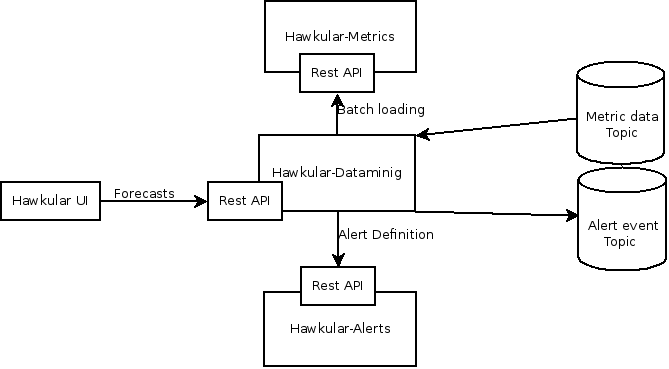
\includegraphics{img/architecture.png}} 
        \caption{Architecture}
        \label{img_arch}
    \end{center}
\end{figure}


%%%%%%%%%%%%%%%%%%%%%%%%%%%%%%%%%%%%%%%%%%%%%%%%%%%%%%%%%%%%%%%%%%% 
\chapter{Evaluation}
%%%%%%%%%%%%%%%%%%%%%%%%%%%%%%%%%%%%%%%%%%%%%%%%%%%%%%%%%%%%%%%%%%% 
\chapter{Conclusion}
\cite{rfc_owamp} %TODO remove

